\documentclass[12pt, a4paper]{article}
\input{/home/mykhailo/.config/nvim/templates/preamble.tex}

\newcommand{\department}{ЗІ}
\newcommand{\reportnumber}{5}
\newcommand{\reporttitle}{Розгортання вебсайту}
\newcommand{\profname}{Синявський О. Ю.}

\begin{document}

\input{/home/mykhailo/Documents/lpnu/report_title_page}
\section{Частина 1: розгортання вебсайту}
Мета --- Навчитися публікувати вебсайт так, щоб він був доступний за публічною адресою в інтернеті. Зрозуміти, як хостинг-платформа підключається до Git-репозиторію, що відбувається під час збірки та як розгорнутий сайт оновлюється сам після кожного коміту. Ознайомитися з різницею між статичним сайтом, який віддається як набір файлів, і застосунком, який перед цим збирається з вихідного коду, а також із налаштуваннями розгортання, що їх розрізняють.
\subsection{Хід роботи}
\begin{enumerate}
	\item Створити акаунт на GitHub
		\begin{itemize}
			\item Створити акаунт на сайті \verb|github.com|.
		\end{itemize}
	\item Створити репозиторій
		\begin{itemize}
			\item Створити порожній публічний репозиторій та завантажити в нього свій вебсайт (папка із кодом).
			\item Додати до лабораторної роботи посилання на репозиторій та його скриншот.
			\item Переконатися, що файл \verb|index.html| міститься в кореневій папці репозиторію.
		\end{itemize}
	\item Розгортання за допомогою Vercel
		\begin{itemize}
			\item Створити акаунт на сайті \verb|vercel.com| та приєднати до нього обліковий запис GitHub.
			\item Створити новий проєкт (\verb|Add New -> Project|) та обрати репозиторій, у якому міститься сайт.
			\item Налаштувати параметри розгортання:
				\begin{itemize}
					\item \verb|Framework Preset| --- \verb|Other|, оскільки фреймворки не використовуються.
					\item \verb|Root Directory| --- тека, в якій міститься \verb|index.html| (корінь репозиторію).
				\end{itemize}
			\item Натиснути \verb|Deploy| та дочекатися повідомлення про успішне розгортання.
			\item Додати до звіту посилання на опублікований сайт та його скриншот.
		\end{itemize}
	\item Оновлення та перевірка
		\begin{itemize}
			\item Зробити будь-які зміни вихідного коду, що змінюють зовнішній вигляд сайту, та закомітити їх.
			\item Додати до лабораторної роботи посилання на коміт.
			\item Переконатися, що після коміту опублікований сайт автоматично оновився.
		\end{itemize}
	\item (Опційно) Власний домен
		\begin{itemize}
			\item Придбати власний домен та спробувати розібратися, як підключити його до свого сайту.
		\end{itemize}
\end{enumerate}
\subsection{Результат}
Репозиторій із вихідним кодом сайту: \url{https://github.com/MykhailoKokhmanskyi/cybersecurity_web_labs}
\begin{figure}[H]
	\centering
	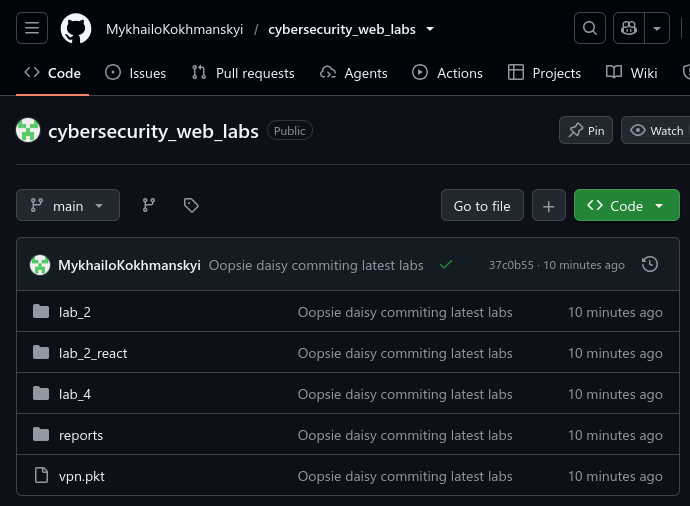
\includegraphics[width=0.7\textwidth]{repo_part1.png}
	\caption{Репозиторій із вихідним кодом сайту на GitHub}
\end{figure}
\begin{figure}[H]
	\centering
	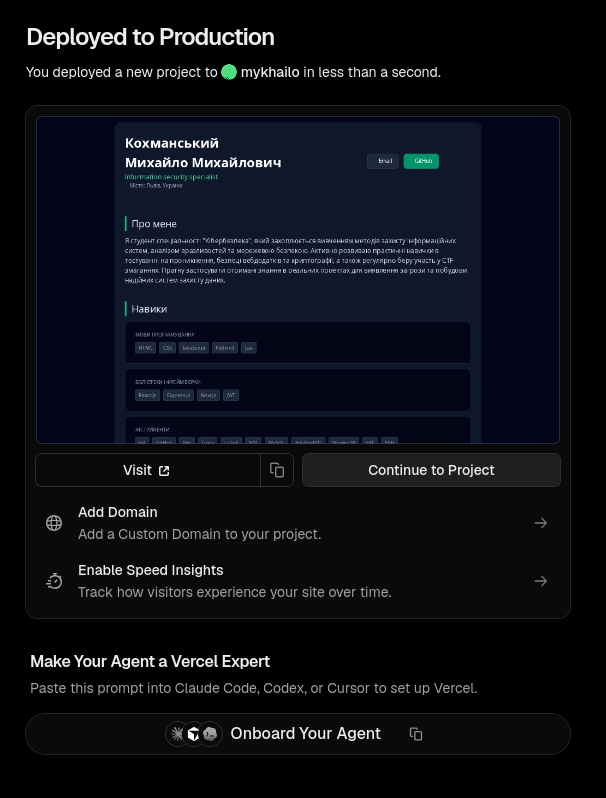
\includegraphics[width=0.7\textwidth]{vercel_success_part1.png}
	\caption{Повідомлення про успішне розгортання сайту}
\end{figure}
Опублікований сайт: \url{https://lab2-one-sage.vercel.app/}
\begin{figure}[H]
	\centering
	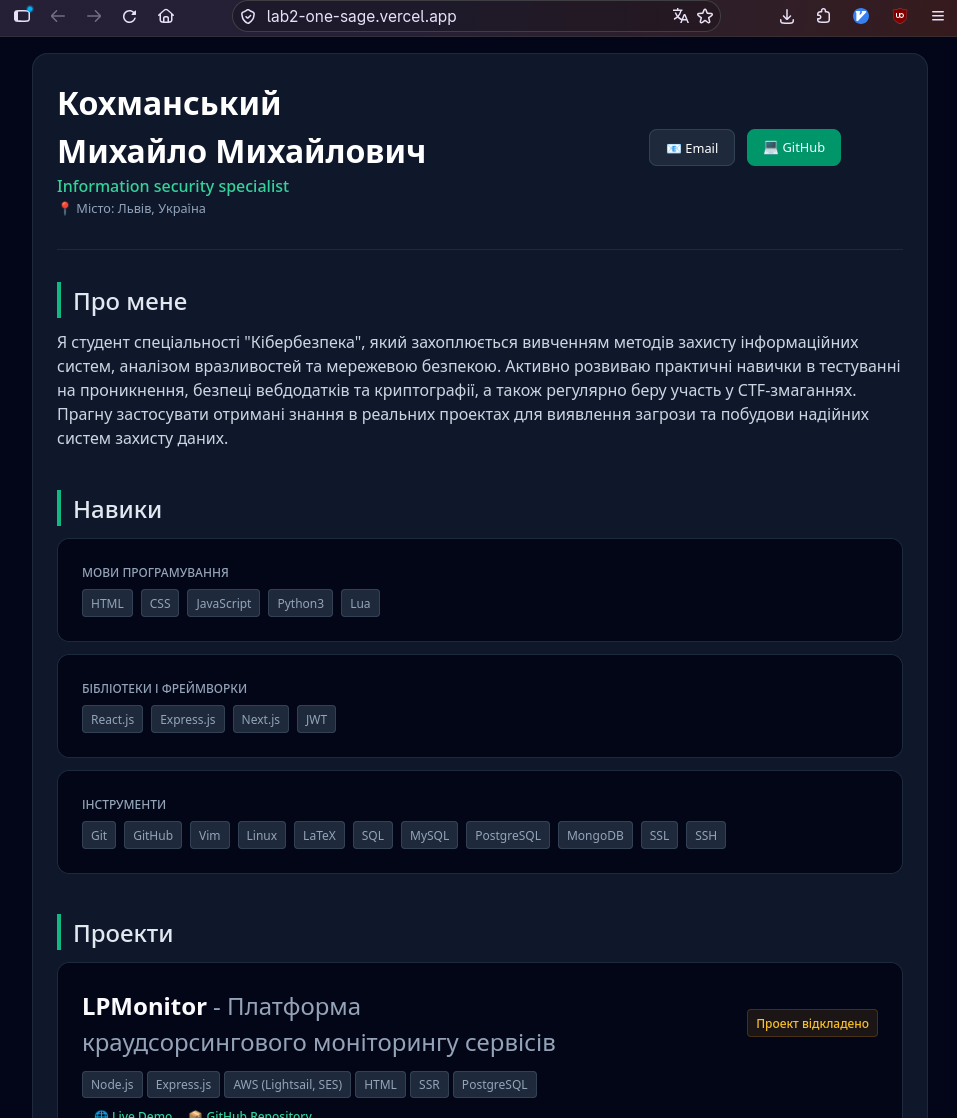
\includegraphics[width=0.7\textwidth]{site_part1.png}
	\caption{Розгорнутий сайт у мережі}
\end{figure}
Коміт зі змінами зовнішнього вигляду сайту: \url{https://github.com/MykhailoKokhmanskyi/cybersecurity_web_labs/commit/7d1e25c0cdfe7f9a1f3369f5f8cad49cf222e499}
\begin{figure}[H]
	\centering
	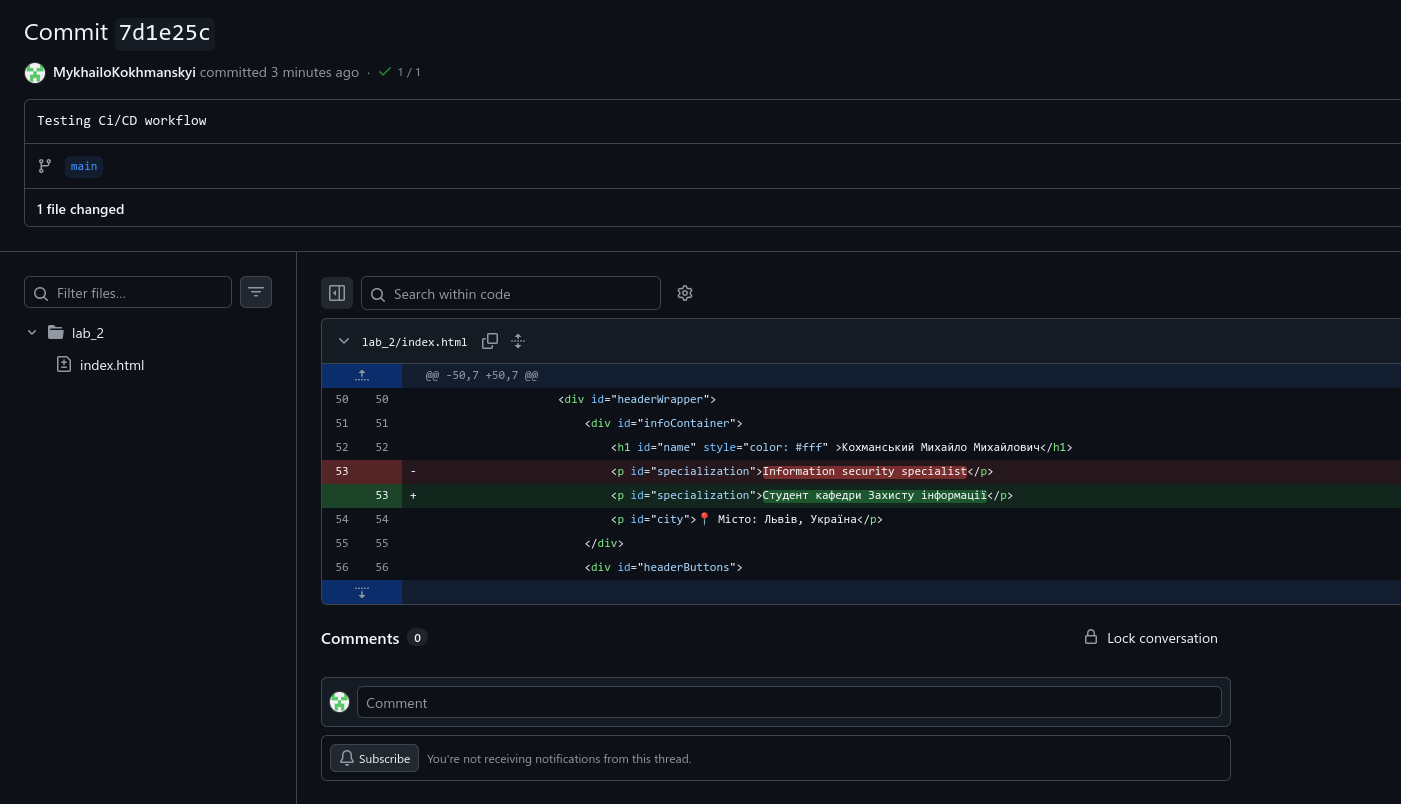
\includegraphics[width=0.7\textwidth]{commit_part1.png}
	\caption{Коміт зі змінами вихідного коду}
\end{figure}
\begin{figure}[H]
	\centering
	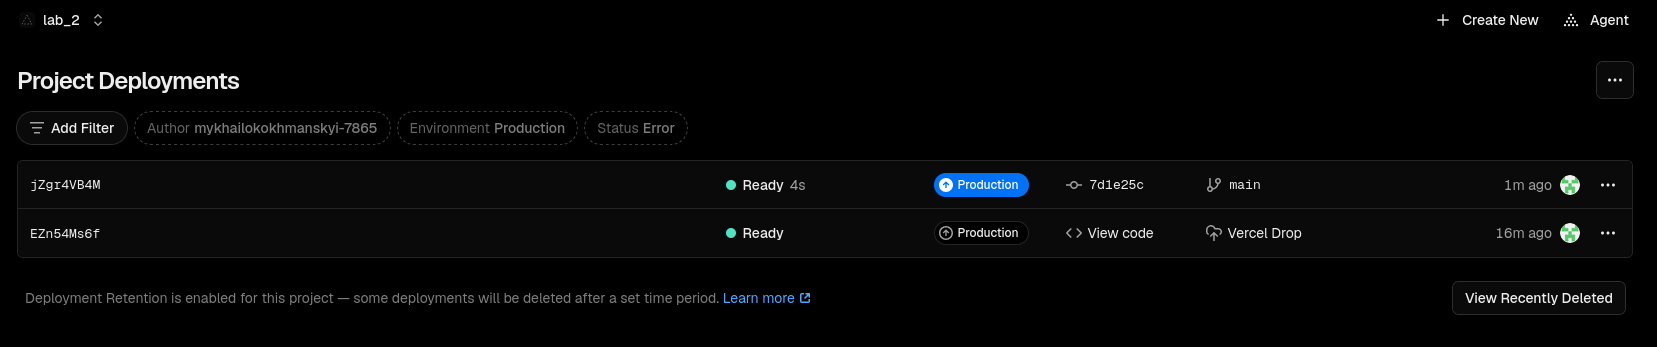
\includegraphics[width=0.7\textwidth]{vercel_deployments_part1.png}
	\caption{Автоматичне розгортання у Vercel після коміту}
\end{figure}
\begin{figure}[H]
	\centering
	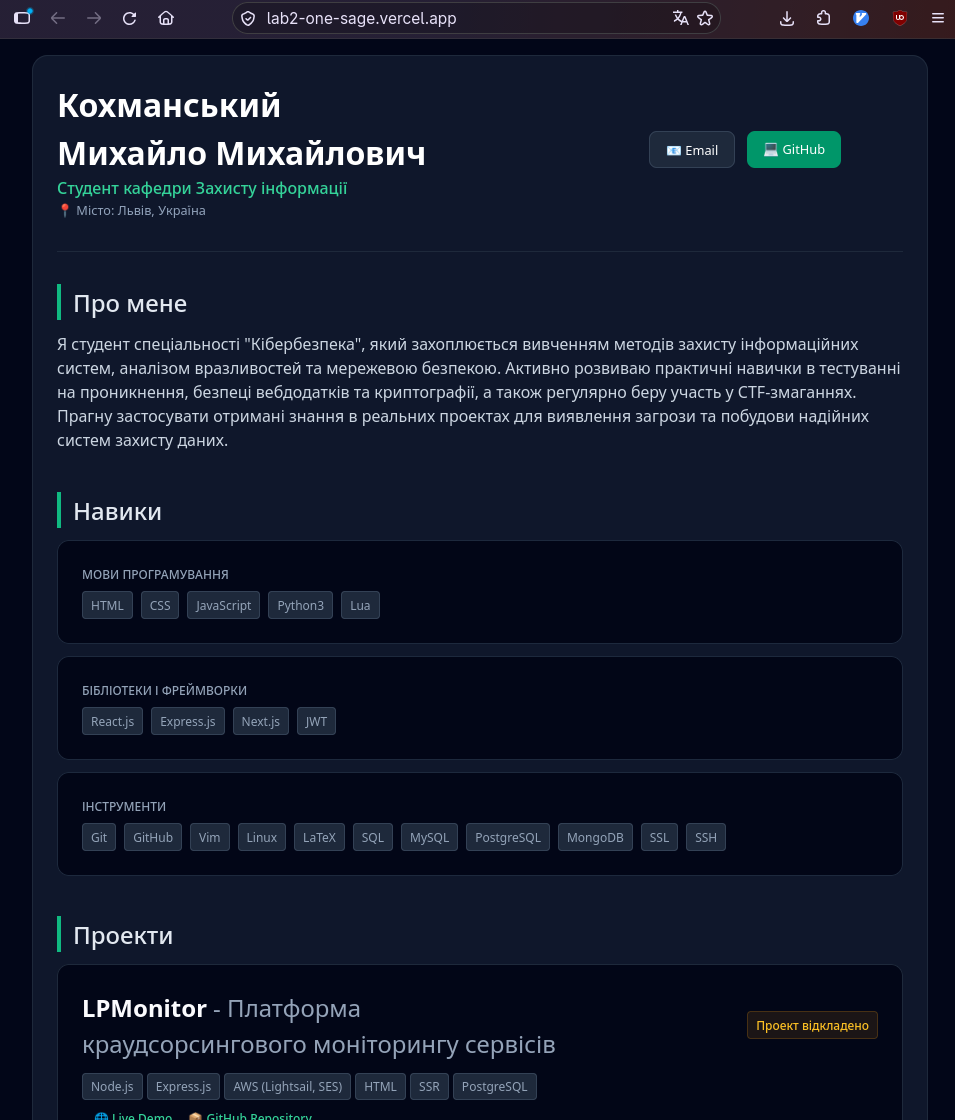
\includegraphics[width=0.7\textwidth]{site_updated_part1.png}
	\caption{Сайт після автоматичного оновлення}
\end{figure}
\section{Частина 2: розгортання React-застосунку}
Мета --- Розгорнути на Vercel React-застосунок, який розвивається з лабораторної роботи №2 (\verb|lab_2_react|).
\subsection{Хід роботи}
\begin{enumerate}
	\item Завантажити код на GitHub
		\begin{itemize}
			\item Переконатися, що проєкт \verb|lab_2_react| містить усі останні зміни (\verb|Footer|, \verb|Reviews|, \verb|ContactForm|, перемикач теми).
			\item Закомітити та завантажити (\verb|push|) зміни у репозиторій на GitHub.
		\end{itemize}
	\item Створити новий проєкт у Vercel
		\begin{itemize}
			\item Перейти на панель керування Vercel та натиснути \verb|Add New -> Project|.
			\item Вибрати репозиторій, який було завантажено у частині 1.
		\end{itemize}
	\item Налаштувати параметри проєкту
		\begin{itemize}
			\item Дати проєкту назву (наприклад, \verb|lab-2-react|).
			\item У розділі \verb|Root Directory| натиснути \verb|Edit| та вибрати теку \verb|lab_2_react| (або інший шлях, за яким React-проєкт лежить у репозиторії).
			\item Переконатися, що \verb|Framework Preset| автоматично визначено як \verb|Vite|.
			\item Перевірити налаштування:
				\begin{itemize}
					\item \verb|Build Command| --- \verb|npm run build| (або \verb|vite build|).
					\item \verb|Output Directory| --- \verb|dist|.
					\item \verb|Install Command| --- \verb|npm install|.
				\end{itemize}
		\end{itemize}
	\item Розгорнути (Deploy)
		\begin{itemize}
			\item Натиснути \verb|Deploy| та дочекатися завершення збірки React-застосунку.
			\item Отримати URL-адресу розгорнутого застосунку.
		\end{itemize}
	\item Подання роботи
		\begin{itemize}
			\item Додати до звіту посилання на розгорнутий React-застосунок.
			\item Додати скриншот розгорнутого застосунку.
		\end{itemize}
\end{enumerate}
\subsection{Результат}
\begin{figure}[H]
	\centering
	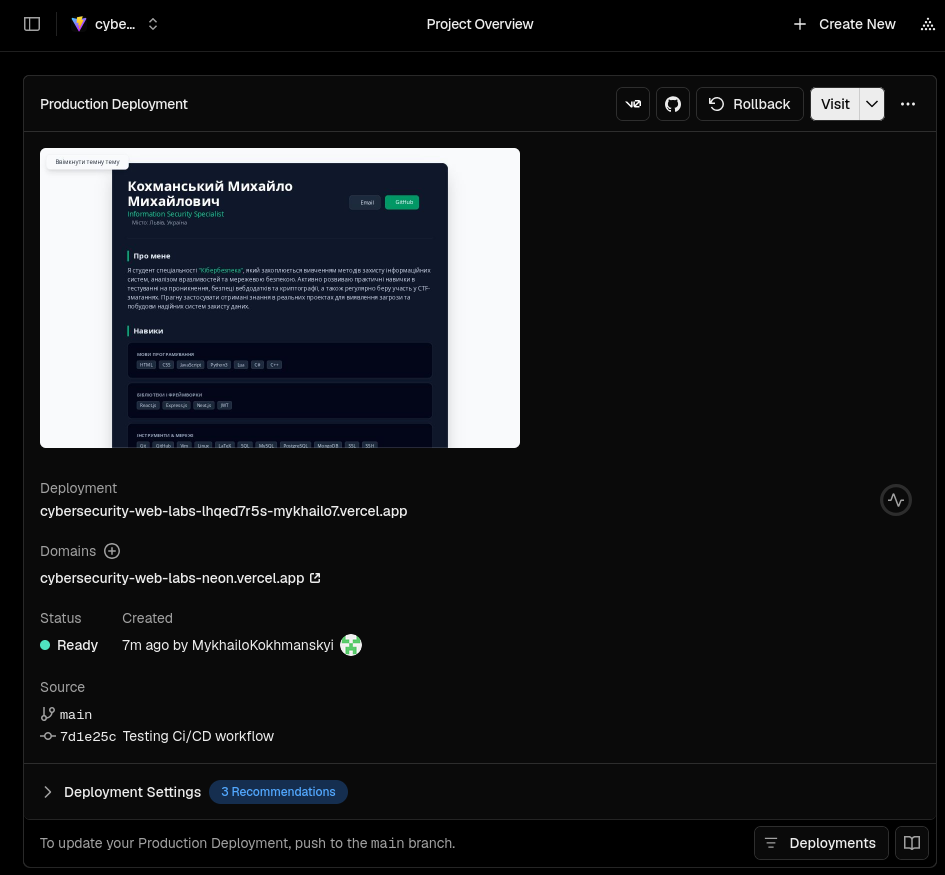
\includegraphics[width=0.7\textwidth]{vercel_part2.png}
	\caption{Проект для React-застосунку у Vercel}
\end{figure}
Розгорнутий React-застосунок: \url{https://cybersecurity-web-labs-neon.vercel.app/}
\begin{figure}[H]
	\centering
	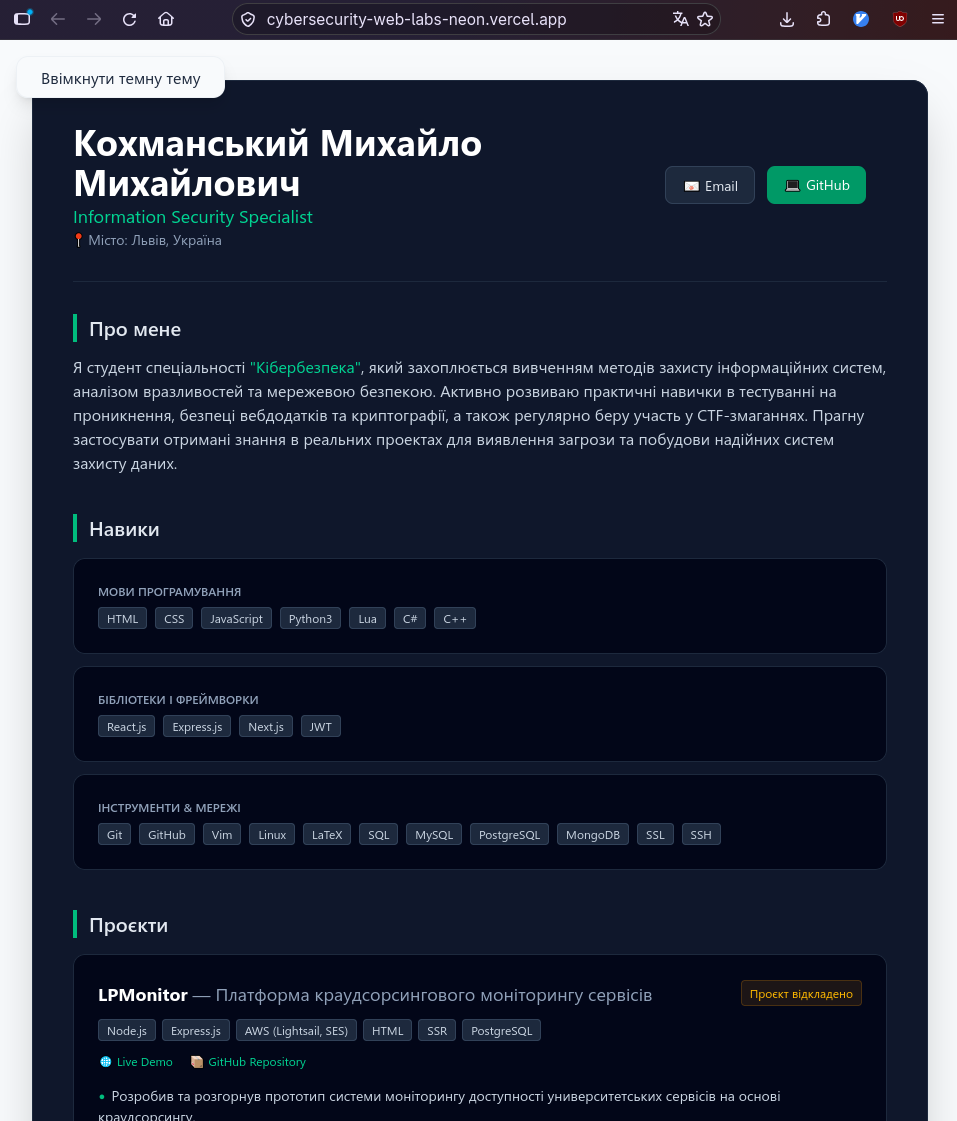
\includegraphics[width=0.7\textwidth]{react_site.png}
	\caption{Розгорнутий React-застосунок у мережі}
\end{figure}
\section{Висновки}
У ході лабораторної роботи було опановано публікацію вебсайту в інтернеті: створено репозиторій на GitHub, підключено його до платформи Vercel та розгорнуто статичний сайт за публічною адресою. Перевірено автоматичне оновлення опублікованого сайту після кожного коміту, а також розглянуто різницю між розгортанням статичного сайту та застосунку, що збирається з вихідного коду. Здобуті знання застосовано на практиці шляхом розгортання React-застосунку \verb|lab_2_react| із коректними налаштуваннями \verb|Root Directory|, \verb|Build Command| та \verb|Output Directory|.
\end{document}
